
\section{Introduction}
\label{sec:introduction}

\begin{figure*}[t]
\centering
\begin{subfigure}[t]{0.49\textwidth}
  \centering
  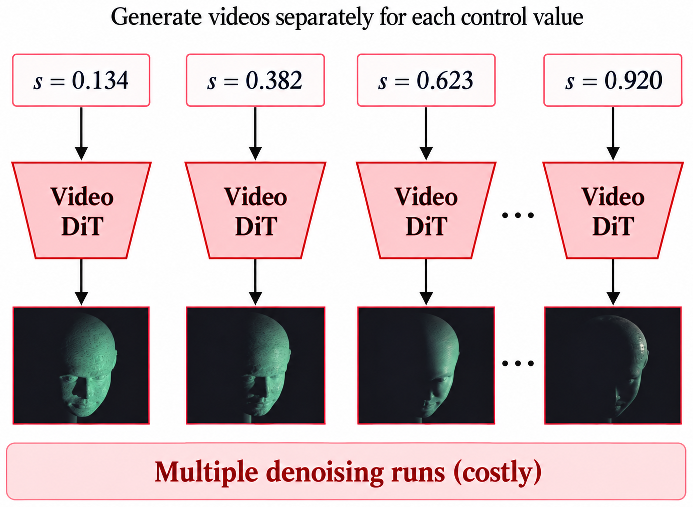
\includegraphics[width=\linewidth]{figures/fig1a_baseline.pdf}
  \caption{Pointwise generation: one diffusion process per control value.}
\end{subfigure}\hfill
\begin{subfigure}[t]{0.49\textwidth}
  \centering
  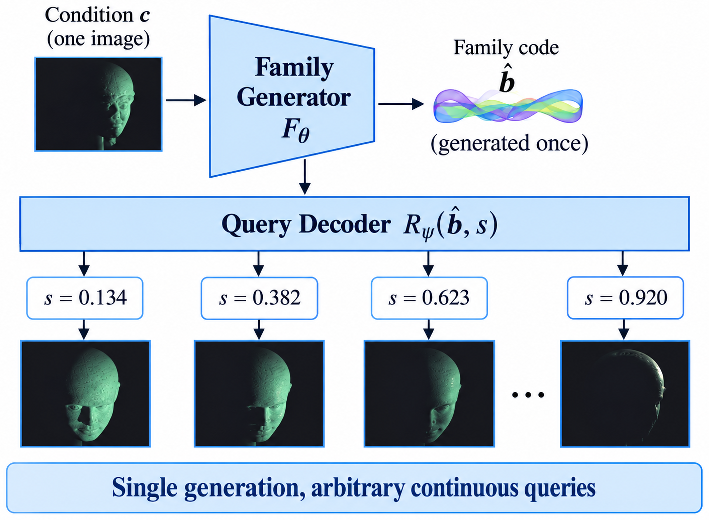
\includegraphics[width=\linewidth]{figures/fig1b_lfvd.pdf}
  \caption{LFVD: one diffusion process, multiple video queries.}
\end{subfigure}
\caption{\textbf{Generate once, query many videos.} Pointwise generation
runs a separate denoising process for each requested control value $s$.
LFVD generates a shared latent representation once and uses a lightweight
query decoder to produce videos at different control values. The thumbnails
show held-out OpenIllumination frames. Multi-query costs are measured in
Sec.~\ref{sec:cost}.}
\label{fig:overview}
\end{figure*}

Video diffusion models have made substantial progress in generating videos
from text and image conditions~\cite{ho2022video,ho2022imagen,singer2022make,
blattmann2023align}. They also support continuous control over video
attributes such as motion intensity and camera speed. In interactive
workflows, users often explore several control values before selecting an
output. These requests may depict the same scene and subject while changing
one attribute. The resulting videos share much of their visual content,
yet generating each video separately repeats expensive computation for
content that is largely unchanged. This motivates reusing information
across control values.

Conventional video diffusion models generate each requested video
separately. Given a control value $s$, the model runs a complete denoising
process to produce the corresponding video. We refer to this approach as
\emph{pointwise generation}. Using the same initial noise can improve
consistency across videos, but the model still performs a separate
denoising process for each control value. Another practical approach
generates videos at selected endpoints and interpolates their latents to
obtain intermediate videos. This reduces repeated sampling, while the
intermediate outputs follow a fixed interpolation rule.

We introduce \textbf{Latent-Function Video Diffusion (LFVD)}, a framework
that generates videos across a continuous control range using a single
diffusion process. LFVD generates a shared latent representation of videos
at different control values. A lightweight query decoder takes this
representation and a requested value $s\in[0,1]$ to produce a complete
video latent, which a frozen video VAE converts into video frames. The
same representation supports multiple queries without additional
denoising. Figure~\ref{fig:overview} illustrates this process.

LFVD learns the shared representation and its generation model in two
stages. First, a frozen video VAE encodes videos observed at different
control values. A family encoder combines their video latents into one
representation, and a query decoder learns to reconstruct each video latent
from the representation and its control value. We train these components
using latent reconstruction loss. Next, we freeze the family encoder and
query decoder and train a pretrained Video DiT to generate shared
representations using standard flow matching. During inference, the Video
DiT samples one representation from the input condition. The query decoder
then produces videos at requested control values without requiring the
original videos or further Video DiT evaluations.

We compare three ways to construct the shared representation.
LFVD-Identity directly concatenates the observed video latents.
LFVD-Mix learns to combine information across latent time and control
positions, while LFVD-Compact uses a shorter representation. All three
use the same query decoder and diffusion training procedure. Their
comparison helps identify how representation design affects generation
quality and computational cost.

The shared representation contains more tokens than a single video latent,
so its diffusion process has a higher initial cost. LFVD can offset this
cost when multiple videos are requested. We measure the trade-off using
synchronized inference time, analytical transformer FLOPs, and
representation-size comparisons.

We evaluate LFVD on lighting and facial-expression control.
OpenIllumination provides measured views of the same objects under
various lights, which we arrange along a fixed camera path to form videos.
MEAD provides facial videos at three ordered expression-intensity levels.
We evaluate on unseen objects and actors and compare with pointwise
generation and interpolation between endpoint video latents.

In lighting control, LFVD improves LPIPS from 0.4000 to 0.3216, PSNR
from 19.29 to 21.14 dB, and control correlation from 0.786 to 0.933
compared with pointwise generation using shared initial noise. LFVD also
generalizes to control values absent from training: with only three
measured lighting positions for training, it improves LPIPS from 0.4103
to 0.3410 at six unseen positions with real measured targets. In
facial-expression control, LFVD maintains video quality comparable to
pointwise generation, although endpoint interpolation achieves stronger
control ordering. Comparisons between LFVD-Identity and LFVD-Mix show
that direct concatenation matches learned mixing overall and provides
better fidelity on MEAD. Synchronized timing shows that LFVD becomes
faster than batched pointwise generation after approximately seven
lighting queries. Together, these results demonstrate the potential
of shared latent representations for efficient video generation
across continuous controls.
\paragraph{Contributions.}
\begin{itemize}
    \item We introduce LFVD, a framework that generates a shared latent
    representation with one diffusion process and uses a lightweight
    query decoder to produce complete videos at continuous control values.
    \item We develop a two-stage training procedure that learns a family
    encoder and query decoder, followed by training a Video DiT using
    standard flow matching.
    \item We evaluate LFVD on lighting and facial-expression control,
    demonstrating video quality, generalization to unseen controls,
    and multi-query efficiency through extensive experiments.
\end{itemize}